\documentclass{beamer}
\mode<presentation>


\usepackage[brazil]{babel}
\usepackage[utf8]{inputenc}
 


\usepackage{amsfonts}
\usepackage{amssymb}
\usepackage{amsmath}
\usepackage{algorithm}
\usepackage{algpseudocode}



\usepackage{ae}
\usepackage{graphicx,color}
\usepackage[all]{xy}
\usepackage{empheq}
\usepackage{fancybox}
\usepackage{textcomp}
\usepackage[all]{xy}
\usepackage{textpos}
\usepackage{multicol}
\usepackage{cancel}
\usepackage{listings}
\usepackage{xcolor}
\usepackage{enumerate}
\usepackage{minted}

\usepackage[style=verbose]{biblatex}
\addbibresource{bibtex.bib}

\usepackage{tikz}
\usetikzlibrary{shapes.geometric, arrows}


\tikzstyle{startstop} = [rectangle, rounded corners, minimum width=3cm, minimum 
\tikzstyle{io} = [trapezium, trapezium left angle=70, trapezium right angle=110, minimum width=3cm, minimum height=1cm, text centered, draw=black, fill=blue!30]
\tikzstyle{process} = [rectangle, minimum width=3cm, minimum height=1cm, text centered, draw=black, fill=orange!30]
\tikzstyle{decision} = [diamond, minimum width=3cm, minimum height=1cm, text centered, draw=black, fill=green!30]
\tikzstyle{arrow} = [thick,->,>=stealth]

\newcommand{\floor}[1]{$\lfloor$ #1 $\rfloor$}

\newcommand\Fontvi{\fontsize{9}{7.2}\selectfont}



\usetheme{Boadilla}

\newcommand{\PC}[1]{\ensuremath{\left(#1\right)}}


\newcommand*{\colorboxed}{}
\def\colorboxed#1#{%
  \colorboxedAux{#1}%
}
\newcommand*{\colorboxedAux}[3]{%
  % #1: optional argument for color model
  % #2: color specification
  % #3: formula
  \begingroup
    \colorlet{cb@saved}{.}%
    \color#1{#2}%
    \boxed{%
      \color{cb@saved}%
      #3%
    }%
  \endgroup
}



\title {Pensando Computacionalmente}

\author[Wladimir Araújo Tavares]{ Wladimir Araújo Tavares$^{1}$  }

\institute[UFC]{$^{1}$Universidade Federal do Ceará - Campus de Quixadá\\}
\date{}
\AtBeginSection[]
{
  \begin{frame}<beamer>{}
    \small
    \tableofcontents[currentsection,currentsubsection]
  \end{frame}
}
\begin{document}

\begin{frame}
	\titlepage
\end{frame}

%%%%%%%%%%%%%%%%%%%%%%%%%%%%%%%%%%%%%%%%%%%%%%%%%%%%%%%%%%%%%%%%%%%%



\begin{frame}{Celebridade}

\begin{itemize}
\item \textbf{Objetivos:} Desenvolver o pensamento computacional.

\item \textbf{Público-alvo:}  Alunos a partir do primeiro ano do Ensino Médio.

\item \textbf{Conteúdo:} Comando de desvio condicional e fluxograma

\item \textbf{Tempo:} 50 minutos

\item \textbf{Recursos:} Papel e Caneta

\end{itemize}
    
\end{frame}




\begin{frame}{Passo 1 - Apresentação da Atividade}

\begin{itemize}
   
\item <1->Nesta atividade, um conjunto de 3 cartões numerados são apresentados para os alunos. Cada um dos cartões representa uma pessoa. Em cada um dos cartões tem um número escrito do outro lado que pode ser 0 indicando que a pessoa não é uma celebridade e 1 indicando que a pessoa é uma celebridade.

\begin{center}
\begin{tikzpicture}
\node[rectangle, draw] (problema) at (0,0){1};
\node[rectangle, draw] (candidato) at (2,0) {2};
\node[rectangle, draw] (teste) at (4,0) {3};

\end{tikzpicture}
\end{center}



\item <2->A tarefa é encontrar a pessoa que é uma celebridade realizando perguntas do tipo "i conhece a pessoa j?".

\item <3-> No nosso problema, uma celebridade é uma pessoa que todos a conhecem e ele não conhece ninguém (meio triste:( ). 



\end{itemize}

\end{frame}


\begin{frame}{Passo 1 - Apresentação da atividade}




\begin{center}
	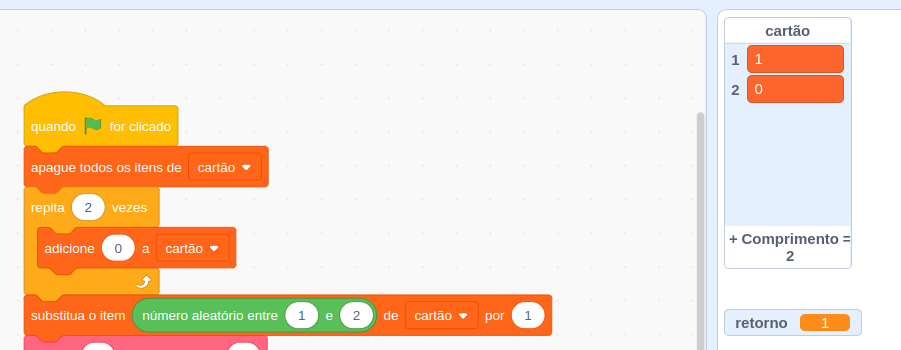
\includegraphics[scale=0.35]{images/inicialização.png} 
\end{center}

    


 



\end{frame}


\begin{frame}{Passo 1 - Apresentação da atividade}




\begin{center}
	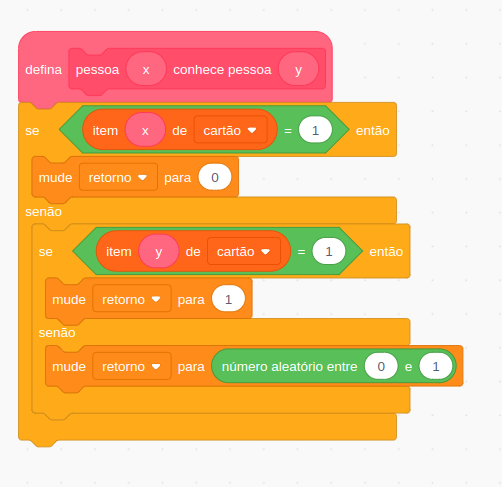
\includegraphics[scale=0.45]{images/perguntas.png} 
\end{center}

    


 

\end{frame}


\begin{frame}{Passo 1 - Apresentação da atividade}




\begin{center}
	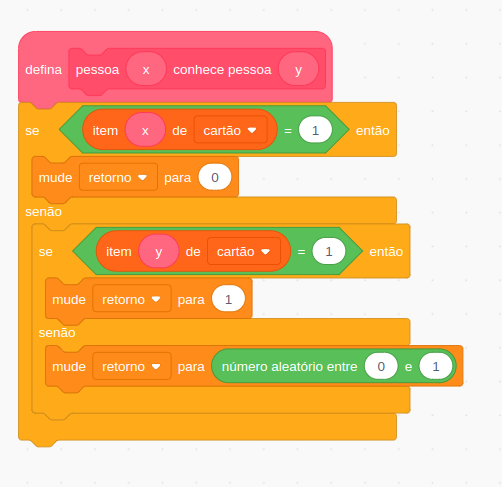
\includegraphics[scale=0.45]{images/perguntas.png} 
\end{center}

    


 

\end{frame}


\begin{frame}{Passo 1 - Apresentação da atividade}


 
    





\end{frame}

\begin{frame}{Passo 1 - Apresentação da atividade}




\begin{center}
	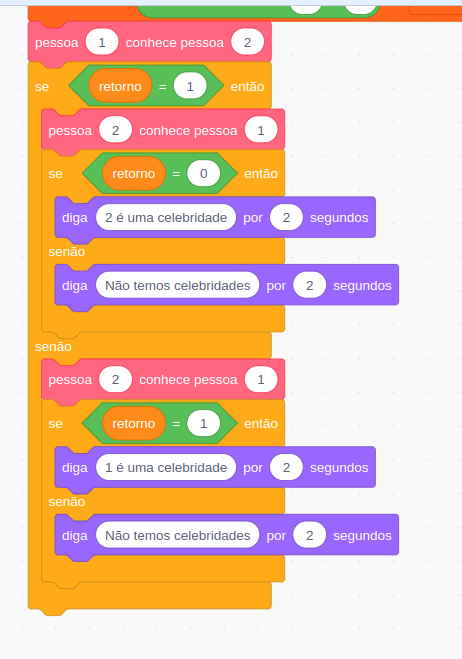
\includegraphics[scale=0.35]{images/jogo.png} 
\end{center}

    


 

\end{frame}


\begin{frame}{Passo 2 - Execução}

\begin{itemize}

\item <1-> A sala pode ser dividade em equipes. Cada equipe deve criar um plano de perguntas a serem realizadas para descobrir quem é a celebridade.

\item <2-> A equipe que está respondendo deve ter enganar a outra equipe. Caso ele consiga enganar a outra equipe, a sua equipe pode ganhar pontos.

\item <4-> Depois, os papéis são invertidos.

\end{itemize}


\end{frame}


\begin{frame}{Passo 3 - Programando no Scratch}

\begin{itemize}

\item Neste passo, os alunos são incentivados a programarem usando a linguagem Scratch.
\end{itemize}


\end{frame}



\begin{frame}{Passo 5 - Discussão e Avaliação}

\begin{itemize}

\item<1-> Os alunos são incentivados a escrever sobre o que eles aprenderam com essa atividade.

\end{itemize}


\end{frame}
% \section{Encontrando o maior}

% \begin{frame}{Tarefa}

% \begin{itemize}

% \item Dado um conjunto de valores, encontre o maior dos valores.

% \begin{center}
% \begin{tabular}{|c|c|c|c|c|}
% \hline
% 10    &  15 & 30 & 42 & 14 \\
% \hline
% \end{tabular}
% \end{center}

% \item Você pode dizer que esse problema é muito fácil e a resposta claramente é 42. 

% \item Como você resolveria esse problema com os olhos fechados e podendo fazer perguntas simples para uma outra pessoa.

% \end{itemize}


% \end{frame}



% \begin{frame}{Decomposição}

% \begin{itemize}

% \item Sabemos que a resposta é o elemento que é maior que todos os outros.

% \item Nesse problema, precisaremos guardar uma informação que chamaremos de candidato, utilizaremos o candidato para comparar com cada um dos valores do nosso conjunto.

% \item Possivelmente, esse candidato pode ser desbancado por um dos valores do nosso conjunto e terá que ser atualizado.


% \end{itemize}


% \end{frame}


% \begin{frame}{Decomposição}


% \begin{tikzpicture}
% \node[rectangle, draw] (problema) at (0,0){Encontrar o maior elemento do conjunto};
% \node[rectangle, draw] (candidato) at (0,-1) {Selecionar um 
% candidato inicial};
% \node[rectangle, draw] (teste) at (1,-3) {Testar se o elemento $i$ desbanca o candidato e atualizar o candidato}; 
% \draw[->]  (problema) -- (candidato);
% \draw[->]  (problema) -- (teste);

% \end{tikzpicture}



% \end{frame}


% \begin{frame}{Reconhecimento de Padrões}


% \begin{itemize}
%     \item O subproblema de testar se um elemento desbanca o candidato atual e atualiza o candidato atual é o mesmo subproblema para todos os elementos do conjunto.
%     \item O que pode mudar entre os testes para cada elemento é que o candidato pode ter sido atualizado.
% \end{itemize}


% \end{frame}


% \begin{frame}{Abstração}


% \begin{itemize}
%     \item Os valores podem ser armazenados em um vetor e podem ser acessados por um índice começado por 1 até o tamanho do conjunto.
%     \item Para realizar o teste e atualização, precisamos acessar o elemento a ser testado e do candidato atual.
% \end{itemize}


% \end{frame}

% \begin{frame}{Algoritmo em pseudocódigo}


% \begin{algorithm}[H]
% \caption{maior\_elemento(A)}
% \begin{algorithmic}
% \Require o tamanho do vetor A deve ser maior que 1.
% \Ensure Devolve o maior elemento do vetor

% \State $candidato \gets A[1]$
% \State $n \gets tamanho(A)$

% \For{$i \gets 1$ \textbf{até} $n$}

% \If{A[i] > candidato}
% \State $candidato \gets A[i]$
% \EndIf

% \EndFor

% \State \Return A[i]

% \end{algorithmic}
% \end{algorithm}

% \end{frame}

% \begin{frame}[fragile]{Algoritmo utilizando a linguagem Python}

% \begin{minted}{Python}[H]
% def maior_elemento(A):
% 	candidato = A[0]
% 	n = len(A)
% 	for i in range(n):
% 		if A[i] > candidato:
% 			candidato = A[i]
% 	return candidato
% if __name__ == "__main__":
% 	print( maior_elemento([4,10,42,15,30]))	

% \end{minted}

% \end{frame}



\end{document}